\documentclass[
	classe=$1^{ere}STI2D$,
	headerTitle=Activité,
]{exercice}

\usepackage{tkz-tab}
\usetikzlibrary{calc}

\setlength{\columnsep}{1cm}

\newcommand{\Repere}[4]{%
	\draw[thin,gray] (#1,#2) grid (#3,#4);
	\draw[thick,->] (#1,0) -- (#3,0);
	\draw[thick,->] (0,#2) -- (0,#4);
	\draw[thick] (1,0) -- ++(0,-0.2) node[below] {$1$};
	\draw[thick] (0,1) -- ++(-0.2,0) node[left] {$1$};
}
\newcommand{\FunctionF}[1]{-0.5*(#1 + 1)*(#1 - 4)}

\title{Activité : tracé d'une fonction de degré 2}

\begin{document}

\maketitle

On définit une fonction $f(x) = -0,5x² + 1,5x + 2$.

\begin{enumerate}
	\item Calculer $f(-4)$ et $f(5)$. \correction{$-12$ et $-3$} \bigskip

	      On admet que le tableau de variations de $f$ est

	      \begin{center}
		      \begin{tikzpicture}
			      \tkzTabInit{$x$ / 1 , $f(x)$ / 2}{$-∞$, $1{,}5$, $+∞$}
			      \tkzTabVar{-/ , +/ \correctionDots{$3{,}125$}, -/ }
		      \end{tikzpicture}
	      \end{center}

	\item Compléter les pointillés ci-dessus.
	\item Sur quel(s) intervalle(s) $f$ est-elle croissante ? \correction{$\intervalle{]}{-∞}{1,5}{]}$}

	      Sur quel(s) intervalle(s) est-elle décroissante ? \correction{$\intervalle{[}{1,5}{+∞}{[}$}
	\item Tracer alors le graphe de la fonction $f$ sur l'intervalle $[-4 ; 5]$ dans le repère ci-dessous :

	      \begin{center}
		      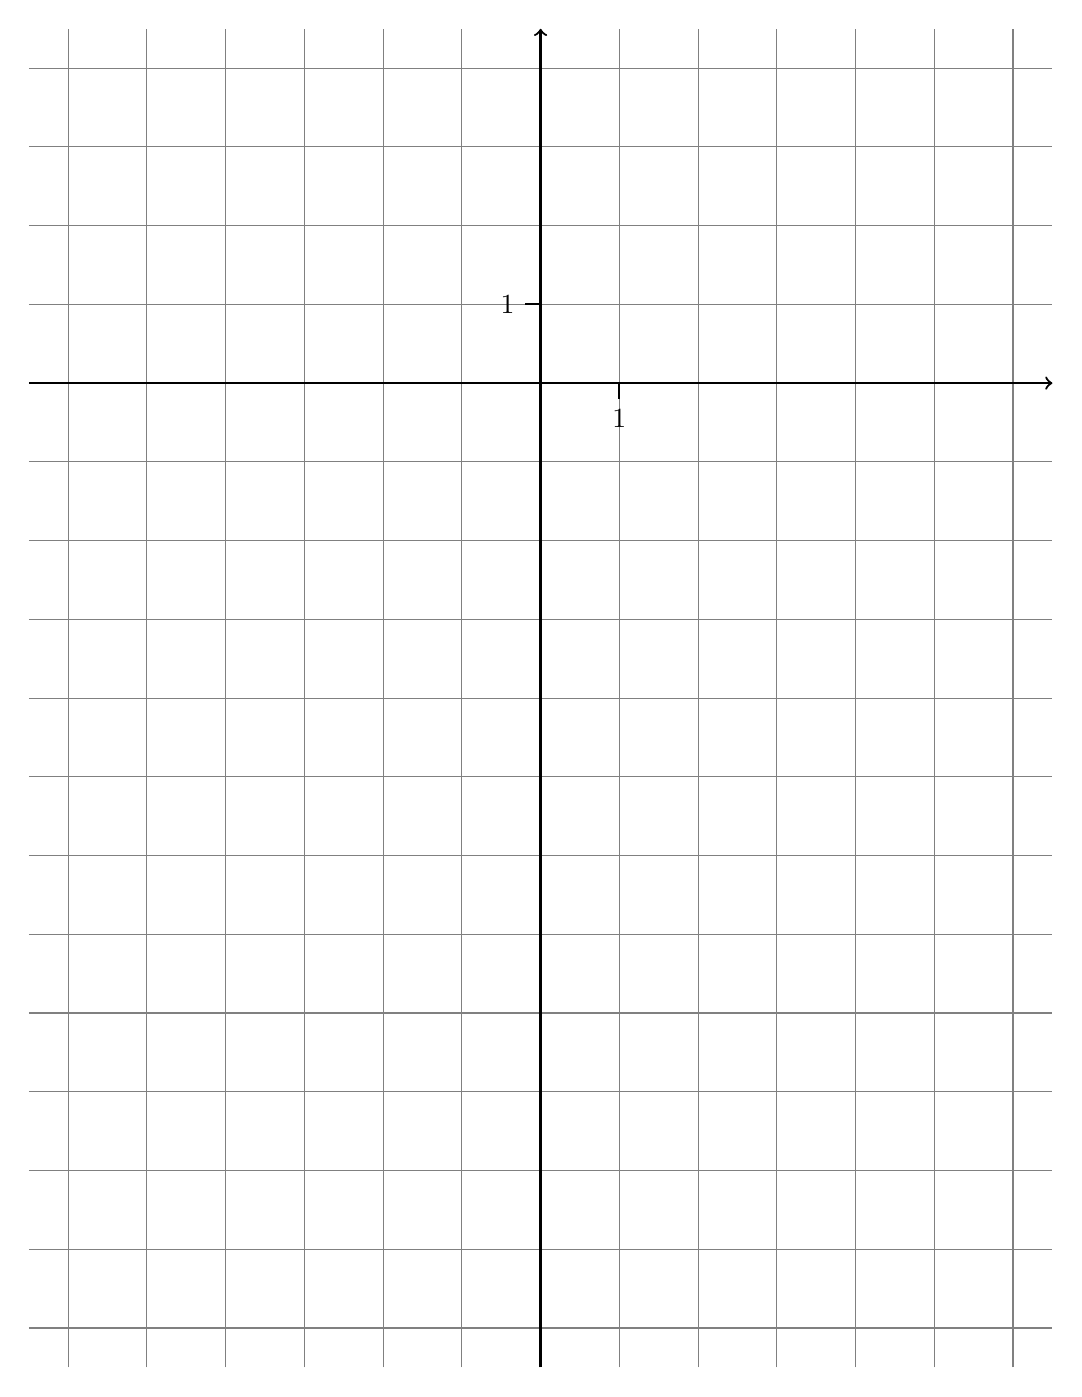
\begin{tikzpicture}
			      \Repere{-6.5}{-12.5}{6.5}{4.5}

			      \ifdefined\makeCorrection
				      \draw[thick,red,variable=\x,domain=-4:5] plot({\x}, {\FunctionF{\x}});
			      \fi
		      \end{tikzpicture}
	      \end{center}
\end{enumerate}

\end{document}